\section{Продуктовое исчисление ширин и размерность 10}
\label{sec:product}

Ширина $d=D/\diam V_0$ до сих пор играла роль отчёта о качестве раскраски: она
говорила, насколько широкий интервал $[1,\ell]$ запрещает построенная
конструкция. Оказывается, у неё есть точный закон сложения, превращающий её в
\emph{расходуемый ресурс}, и одного этого хватает, чтобы улучшить оценку в
размерности~10.

\subsection{Правило сложения}
\label{ssec:prodrule}

\begin{proposition}[продуктовое исчисление]\label{prop:product}
Пусть $\Lambda=\bigoplus_{i=1}^{s}\Lambda_i$ --- ортогональная прямая сумма
решёток $\Lambda_i\subset\R^{n_i}$, и $\Gamma=\bigoplus_i\Gamma_i$ с
$\Gamma_i\subseteq\Lambda_i$. Обозначим $d_i=D_{\min}(\Gamma_i)/\diam V_0(\Lambda_i)$
и $k_i=[\Lambda_i:\Gamma_i]$. Тогда раскраска по $\Gamma$ допустима для интервала
$[1,\ell]$ с
\[
\ell=\Bigl(\sum_i 1/d_i^2\Bigr)^{-1/2},
\]
в частности она даёт $\chi(\R^{n},[1,\ell])\le\prod_i k_i$, $n=\sum_i n_i$, как
только $\sum_i 1/d_i^2\le1$. Оптимум достигается при
$\diam V_0(\Lambda_i)^2\propto 1/d_i^2$.
\end{proposition}

\begin{proof}
Ячейка Вороного прямой суммы есть произведение ячеек, поэтому
$\diam^2 V_0(\Lambda)=\sum_i\diam^2 V_0(\Lambda_i)$. Далее, для
$v=(v_1,\dots,v_s)$ имеем $\dist(v/2,V_0)^2=\sum_i\dist(v_i/2,V_0(\Lambda_i))^2$,
то есть $D(v)^2=\sum_i D_i(v_i)^2$. Так как $D_i(0)=0$, минимум по
$\Gamma\setminus\{0\}$ достигается на векторе с единственной ненулевой
компонентой, и условие допустимости $D_{\min}\ge\ell\diam V_0$ распадается на
$s$ условий
\[
d_i^2\,s_i\ \ge\ \ell^2\sum_j s_j,\qquad s_i:=\diam^2 V_0(\Lambda_i).
\]
Блоки можно масштабировать независимо, поэтому положим $s_i=S/d_i^2$; тогда
каждое условие обращается в равенство при $\ell^2=S/\sum_j s_j
=\bigl(\sum_j 1/d_j^2\bigr)^{-1}$. Любой другой выбор $s_i$ даёт не большее
$\ell$: минимум по $i$ величины $d_i^2 s_i/\sum_j s_j$ максимизируется именно при
пропорциональности.
\end{proof}

При $\Gamma_i=3\Lambda_i$ имеем $d_i=2/\rho_i$ и правило превращается в известное
$\sum_i\rho_i^2\le4$ (предложение~\ref{prop:mult}). Существенно, однако, что
в общей форме блоки могут иметь \emph{разный индекс}: именно смесь дорогого
широкого блока с дешёвым узким и работает.

\subsection{\texorpdfstring{$\alpha$}{alpha}-лестница}
\label{ssec:alphaladder}

Чтобы правило было применимо, для каждой размерности нужна лестница пар
$(k,d)$. Одно семейство даёт её в замкнутой форме сразу для всех порядков,
действующих подобиями.

\begin{proposition}[$\alpha$-лестница]\label{prop:alphaladder}
Пусть $\mathcal R\in\{\Z,\Z[i],\Z[\omega],\mathcal H\}$ ($\mathcal H$ ---
кватернионы Гурвица), $\Lambda\subset\R^n$ --- модуль над $\mathcal R$, и
$\alpha\in\mathcal R$. Тогда $\Gamma=\alpha\Lambda$ имеет индекс $|\alpha|^n$ и
\[
D(\alpha w)\ \ge\ 2\,|w|\cdot\dist\bigl(\alpha/2,\ U\bigr)\quad\text{для всех }w\in\Lambda,
\]
где $U$ --- ячейка Вороного решётки $\mathcal R w$ при $|w|=1$: отрезок, квадрат,
шестиугольник или 24-ячейка. Как следствие
$d\ge 2\dist(\alpha/2,U)/\rho$, $\rho=\diam V_0/\lambda_1$.
\end{proposition}

Доказательство дословно повторяет планарную теорему
(предложение~\ref{prop:planar}): единицы $\mathcal R$ дают равнонормные векторы
$uw$, чьи опорные полупространства лежат \emph{внутри} линейной оболочки
$\mathcal R w$, поэтому проекция $V_0$ на неё содержится в $U$, а расстояние
считается уже в этой оболочке.

Вещественный множитель даёт $\dist(m/2,[-1/2,1/2])=(m-1)/2$, то есть
$d=(m-1)/\rho$; эйзенштейнов $3+\omega$ даёт $\sqrt{7/12}$, то есть
$d=\sqrt{7/3}/\rho$. Отметим совпадение: кватернион Гурвица нормы~7, например
$2+i+j+k$, даёт \emph{ровно ту же} константу $\sqrt{7/12}$, а норма~8
(элемент $2+2i$) --- константу $\sqrt{1/2}$, то есть требует $\rho\le\sqrt2$ при
индексе $8^{n/2}=2{,}828^n$.

\subsection{Размерность 10: индекс 45619}
\label{ssec:dim10}

\begin{theorem}\label{thm:dim10}
$\displaystyle\chi\Bigl(\R^{10},\bigl[1,\sqrt{217/214}\bigr]\Bigr)\ \le\ 2401\cdot19=45619.$
\end{theorem}

\begin{proof}
Берём два блока.

\emph{Блок $E_8$.} $\Gamma_1=(3+\omega)E_8$, индекс $7^4=2401$. При нормировке
$\lambda_1^2=3$ имеем $\diam^2 V_0=6$, а $D_{\min}=\sqrt7$: неравенство
$\ge$ --- планарная теорема, равенство достигается на минимальных векторах.
Значит $d_1^2=7/6$ и цена блока $1/d_1^2=6/7$.

\emph{Плоский блок.} $\Gamma_2=(5+2\omega)\,aA_2$, индекс $N(5+2\omega)=19$.
В плоскости ячейка Вороного \emph{и есть} шестиугольник, поэтому величина $D$
здесь точна, а не оценена: ближайшая к точке $(5+2\omega)/2=(2,\sqrt3/2)$ точка
шестиугольника --- его вершина $(1/2,1/(2\sqrt3))$, расстояние до неё равно
$\sqrt{31/12}$. Отсюда $D_{\min}=2a\sqrt{31/12}$, $\diam V_0=2a/\sqrt3$ и
$d_2^2=31/4$, цена $1/d_2^2=4/31$.

Сумма цен $6/7+4/31=214/217<1$, и предложение~\ref{prop:product} даёт
$\ell=\sqrt{217/214}$ при $\prod k_i=2401\cdot19=45619$.
\end{proof}

Прежняя оценка в этой размерности --- $3^{10}=59049$ (башня
ламинаций, \S\ref{ssec:tower}), так что выигрыш составляет $22{,}7\%$. Оптимальный
масштаб плоского блока $a=\sqrt7/(2\sqrt{31/12})=0{,}8230549$; сквозная проверка
построенной решётки в $\R^{10}$ подтверждает индекс ровно $45619$,
$D_{\min}=2{,}645751311$, $\diam=2{,}627399057$ и $d=1{,}006984951$, что
совпадает с $\sqrt{217/214}$ до $10^{-9}$.

\begin{figure}[htbp]\centering
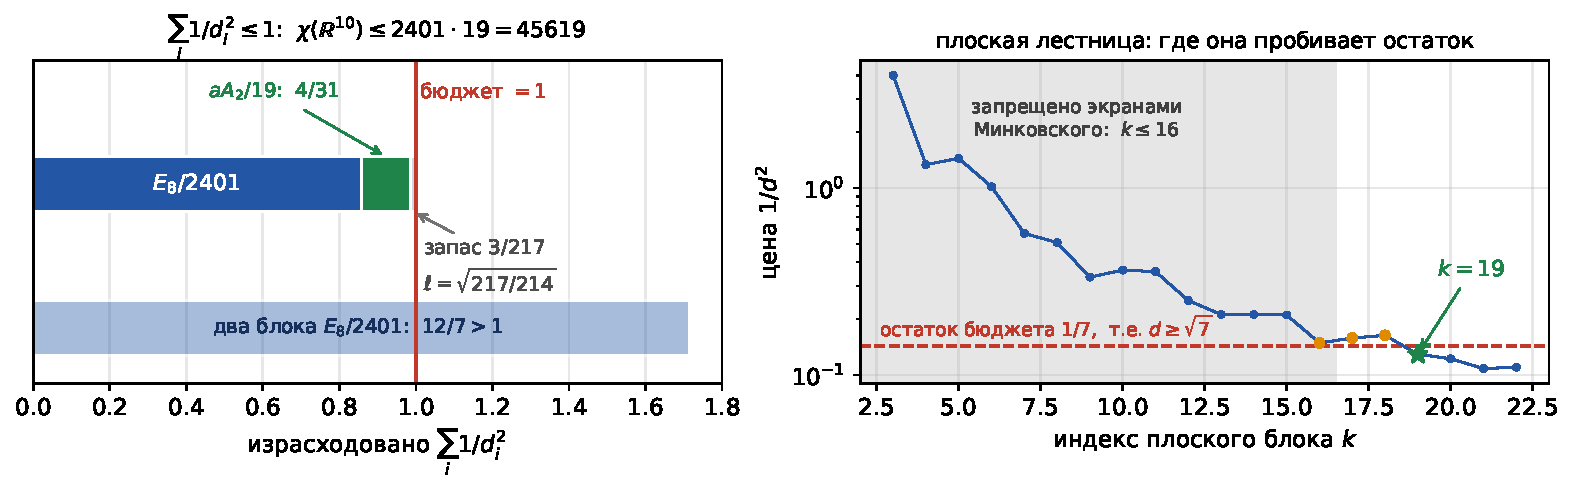
\includegraphics[width=\textwidth]{fig_budget.pdf}
\caption{Слева: бюджет $\sum_i 1/d_i^2\le1$ как полоса длины~1. Блок $E_8/2401$
занимает $6/7$, плоский проставок индекса~19 --- $4/31$, остаток $3/217$ и даёт
ширину $\ell=\sqrt{217/214}$. Два блока $E_8/2401$ в бюджет не помещаются
($12/7>1$) --- поэтому в произведении может быть лишь один эффективный блок.
Справа: плоская лестница цены $1/d^2$ по индексу; горизонталь --- остаток
бюджета $1/7$, серая зона запрещена экранами (\S\ref{ssec:planefloor}).}
\label{fig:budget}
\end{figure}

\subsection{Плоский блок индекса 19 неулучшаем}
\label{ssec:planefloor}

Рядом с $E_8/2401$ плоский блок обязан иметь $d\ge\sqrt7$. Полный перебор
показывает, что впервые это достигается при $k=19$: перебираются все формы
Эрмита индекса~$k$ (их $\sigma(k)$) и все формы плоских решёток с точностью до
подобия (двупараметрическое семейство; максимизация численная). Индексы
$16,17,18$ дают $2{,}598$, $2{,}520$, $2{,}479$.

Нижняя часть диапазона закрывается доказательно, причём двумя дополняющими
экранами. Первый --- объёмный (\S\ref{ssec:mink}): $k\ge\vol(V_0\oplus
(\ell\diam/2)B)/\det\Lambda$, что на шестиугольной решётке даёт $15{,}574$.
Второй новый.

\begin{proposition}[инрадиусный экран]\label{prop:inrfloor}
Для допустимой при ширине $\ell$ пары $\Gamma\subset\Lambda\subset\R^n$
\[
k=[\Lambda:\Gamma]\ \ge\ \frac{(\ell\,\diam V_0+\lambda_1)^n}
{\gamma_n^{n/2}\,\det\Lambda}.
\]
\end{proposition}

\begin{proof}
Инрадиусная лемма~\ref{lem:inradius} даёт $D(v)\le|v|-\lambda_1$, поэтому
допустимость влечёт $\lambda_1(\Gamma)\ge\ell\diam V_0+\lambda_1$. Неравенство
Эрмита $\lambda_1(\Gamma)^n\le\gamma_n^{n/2}\det\Gamma$ и
$\det\Gamma=k\det\Lambda$ дают требуемое.
\end{proof}

Этот экран \emph{не следует} из объёмного и в плоскости при $\ell=\sqrt7$
сильнее: $16{,}443$ против $15{,}574$ на шестиугольной решётке. Оба верны для
каждой формы решётки, поэтому строгий пол есть минимум по формам от максимума
двух экранов; скан пространства модулей с последующей доводкой даёт $16{,}021$
(при $x=-0{,}5$, $y=1{,}0754$). Итог: \emph{индекс $k\le16$ невозможен
доказательно}, а $k=17,18$ исключены пока лишь численно.

\begin{figure}[htbp]\centering
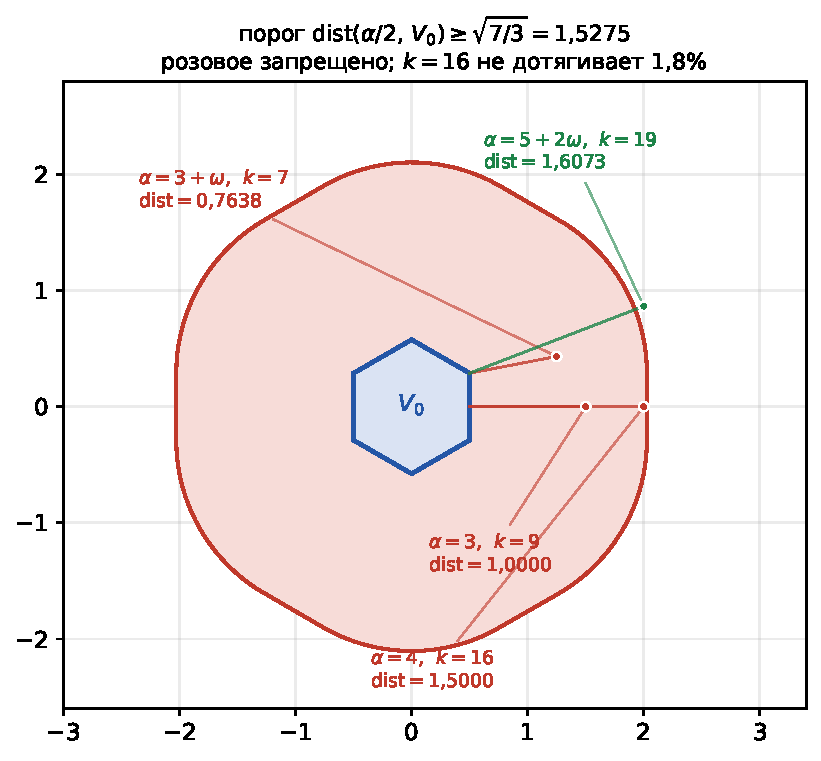
\includegraphics[width=0.72\textwidth]{fig_spacer.pdf}
\caption{Почему плоский проставок стоит ровно~19. Синий шестиугольник --- ячейка
$V_0$ решётки $A_2$; розовая область --- её окрестность радиуса
$\sqrt{7/3}=1{,}5275$, куда точка $\alpha/2$ попадать не должна. Отрезки ведут к
ближайшей точке ячейки. Индекс~16 ($\alpha=4$) не дотягивает $1{,}8\%$, и лишь
$\alpha=5+2\omega$ выходит наружу.}
\label{fig:spacer}
\end{figure}

\subsection{Лестницы и динамика по разбиениям}

Собрав лестницы (замкнутые $\alpha$-лестницы для четырёх порядков плюс
сертифицированные результаты настоящей работы) и минимизировав $\prod_i k_i$ при
ограничении $\sum_i 1/d_i^2\le1$ динамическим программированием по разбиениям
$n=\sum n_i$, получаем таблицу, которая \emph{воспроизводит все известные
рекорды} ($n=4{:}45$, $5{:}132$, $6{:}343$, $7{:}1029$, $8{:}2401$, $9{:}7203$,
$12{:}3^{12}$, $24{:}7^{12}$) --- это её проверка --- и добавляет три значения:
\[
n=10{:}\ 45619,\qquad
n=25{:}\ 4\cdot7^{12},\qquad
n=26{:}\ 19\cdot7^{12},
\]
последние два в $15{,}3$ и $9{,}7$ раза лучше $3^n$. Дальше произведения не
помогают: блок $E_8/2401$ расходует $6/7$ бюджета, поэтому эффективный блок в
произведении может быть только один.

\subsection{Теорема о бюджете слоя}
\label{ssec:layerbudget}

Ламинирование \S\ref{ssec:lam} надстраивает по одному измерению слоями $t\Z$.
Прямая --- худшее из возможных покрытий, и естественно заменить её слоевой
\emph{решёткой}.

\begin{proposition}[бюджет слоя]\label{prop:layerbudget}
Пусть база $(\Lambda_0,\Gamma_0)$ имеет ширину $d_0$ и диаметр $\diam_0=2R_0$, и
пусть $\Lambda$ получена ламинированием слоевой решёткой $L\subset\R^m$ с
радиусом покрытия $R_L$ и произвольными поправками. Тогда
$\diam V_0(\Lambda)\le2\sqrt{R_0^2+R_L^2}$ и горизонтальные разделения
сохраняются, поэтому горизонтальная часть условия выполнена, как только
\[
R_L\ \le\ \frac{\diam_0}{2}\sqrt{d_0^2-1}.
\]
\end{proposition}

Иначе говоря, \emph{избыток ширины раскраски есть в точности бюджет радиуса
покрытия на дополнительные измерения}. Для $E_8/2401$ ($\diam_0=\sqrt6$,
$d_0^2=7/6$) бюджет равен ровно $R_L\le1/2$, и обе известные строгие ступени
оказываются двумя способами его потратить: одна прямая единичной высоты даёт
$\R^9$ с индексом $2401\cdot4=9604$, один шестиугольник с $\lambda_1=\sqrt3/2$
даёт $\R^{10}$ с индексом $2401\cdot19=45619$.

Конструкцию полезно делать $\Z[\omega]$-эквивариантной: $\omega$ переставляет три
минимальных направления $A_2$, поэтому вместо трёх независимых слоевых условий
остаётся одна орбита, а свободных параметров --- восемь вместо шестнадцати. На
практике это подняло численный фронтир с $0{,}85$ до $0{,}966$ при том же
бюджете поиска.

\subsection{Что закрыто отрицательно}
\label{ssec:prodneg}

\textbf{$7^6$ в размерности 12 недостижимо.} Планарная теорема даёт лишь нижнюю
оценку $D\ge\sqrt{7/3}\lambda_1$, и оставался шанс, что у решётки Коксетера--Тодда
настоящее $D$ больше (тогда $\chi(\R^{12})\le7^6=117649$ вместо $3^{12}=531441$).
Прямой счёт закрывает вопрос: перебор $85\,680$ векторов $(3+\omega)K_{12}$
против полупространств \emph{всех} $756$ минимальных векторов даёт
$D_{\min}=3{,}055050463$ --- ровно планарный пол, при требуемом
$\diam=2\sqrt{8/3}=3{,}265986$. Причина видна: вершину шестиугольника могли бы
отсечь только векторы нормы $<1{,}1547\lambda_1$, а у $K_{12}$ таких нет. Значит
эйзенштейнов путь в $\R^{12}$ требует именно $\rho\le\sqrt{7/3}=1{,}5275$, тогда
как $\rho(K_{12})=1{,}6330$.

\textbf{Слой ранга 2 не проходит.} Естественное продолжение --- надстроить над
$E_8/2401$ слоевую решётку ранга~2, получив $\chi(\R^{12})\le2401\,N(\alpha)^2$.
Попутно найдена лучшая эйзенштейнова решётка ранга~2: оптимизация по эрмитовым
формам даёт $\rho=1{,}3626553$, что лучше $D_4$ ($\sqrt2$) и $A_2\oplus A_2$
($1{,}6330$). Тем не менее фронтир встаёт на $0{,}79$--$0{,}94$, причём
пятикратное увеличение бюджета оптимизации ухудшает результат: ландшафт рваный.

Причина установлена подсчётом и показана на рис.~\ref{fig:shells}: поправки
обязаны вытолкнуть за диаметр \emph{каждый} класс слоевой подрешётки, попавший
в окно $|c|\le\diam+\lambda_1$. В плоскости таких классов ровно шесть --- одна
орбита действия $\omega$, а следующая оболочка лежит далеко за окном; в ранге~2
их двадцать четыре, четыре орбиты, причём три почти вырождены по длине
($3{,}2909$, $3{,}2913$, $3{,}2916$) и должны быть вытолкнуты одновременно.
Отсюда видна тензия, которую иначе нечем было бы заметить: малое $\rho$ означает
<<круглую>> решётку, а круглая решётка имеет много векторов почти равной длины,
то есть много связывающих орбит. Слою нужны одновременно малое~$\rho$ (бюджет)
и разреженные оболочки (выполнимость), и в ранге~1 второе даётся даром.

\begin{figure}[htbp]\centering
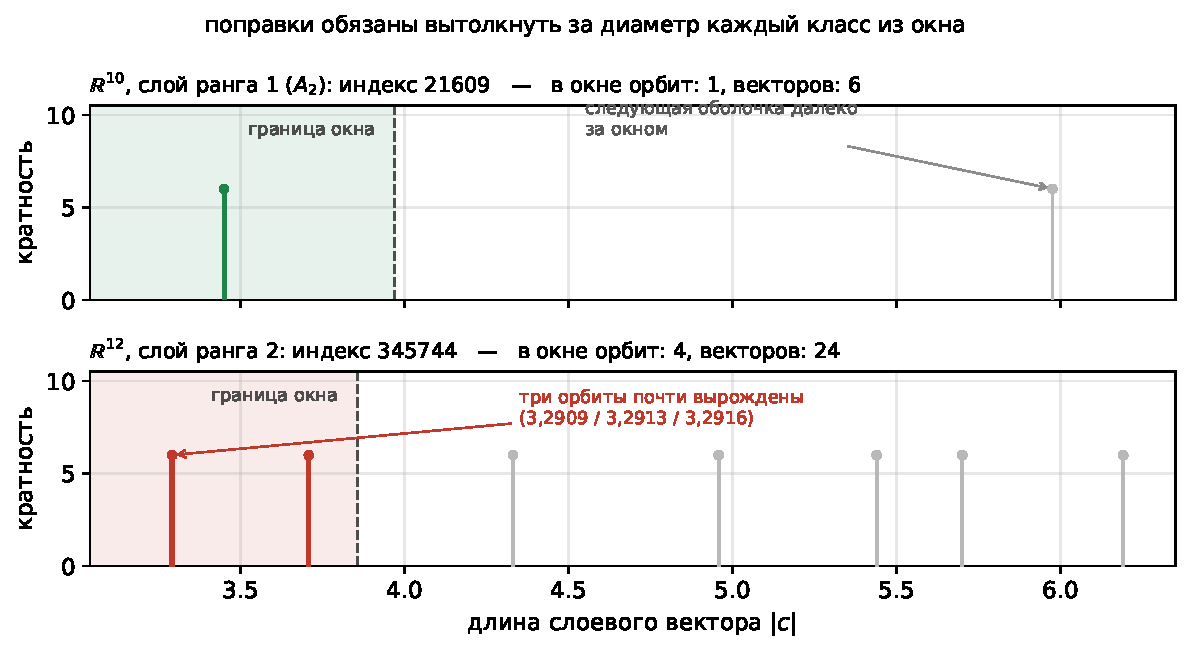
\includegraphics[width=\textwidth]{fig_shells.pdf}
\caption{Длины слоевых векторов подрешётки с кратностями. Сверху слой ранга~1
(размерность~10): в окне одна орбита, следующая оболочка далеко. Снизу слой
ранга~2 (размерность~12): четыре орбиты, три почти вырождены.}
\label{fig:shells}
\end{figure}

\textbf{$E_8$ --- локальный минимум $\rho$.} Поскольку узким местом оказался
разрыв восьмимерной лестницы между $2401$ ($d=1{,}0801$) и $6561$
($d=1{,}4142$), естественно спросить, нельзя ли поднять ширину самого блока,
взяв другую эйзенштейнову решётку. Отображение выигрыша прямое,
$d=\sqrt{7/3}/\rho$, и пороги в $\R^{10}$ таковы: $\rho\le1{,}4099$ даёт
проставок индекса~16 и оценку $38416$; $\rho\le1{,}3581$ --- индекс~13 и
$31213$; $\rho\le1{,}3229$ --- индекс~12 и $28812$; $\rho\le1{,}2472$ ---
индекс~9 и $21609$. У $E_8$ ровно $\rho=\sqrt2=1{,}4142$, до первого порога не
хватает $0{,}3\%$, а объёмный пол упаковки $(1/\delta_8)^{1/8}=1{,}1868$ ничего
из этого не запрещает. Тем не менее ответ отрицательный: $E_8$ восстанавливается
из своего $\Z[\omega]$-базиса ($\rho=1{,}414213562$ ровно), и локальная
оптимизация из неё даёт только худшие значения --- $1{,}4198$, $1{,}4237$,
$1{,}4243$, $1{,}4241$ при малом шаге и $1{,}4602$, $1{,}4408$, $1{,}4351$,
$1{,}4374$ при большом. Разрыв восьмимерной лестницы придётся брать
неэйзенштейновыми подрешётками, а не деформацией родительской решётки.

\subsection{Кандидаты в размерности 10}
\label{ssec:dim10cand}

За пределом границы $\diam\le2\sqrt{R_0^2+R_L^2}$ измеренный диаметр
оказывается заметно меньше её, и индекс падает. Как и в случае $7203$
(\S\ref{ssec:7203}) до появления сертификата, статус этих конструкций ---
\emph{численный}:
\[
\begin{array}{r|c|c|c|c}
\text{индекс} & N & a & D_{\min} & d\ \text{(измер.)}\\\hline
38416 & 16 & 0{,}90 & 2{,}6457513 & 1{,}0616\\
28812 & 12 & 0{,}95 & 2{,}6457513 & 1{,}0521\\
21609 & 9  & 1{,}15 & 2{,}6457513 & 1{,}0093
\end{array}
\]
Нижняя строка --- $21609=3^2\cdot7^4$, в $2{,}73$ раза ниже $3^{10}$. Во всех
трёх $D_{\min}$ упирается ровно в $\sqrt7$: слоевые векторы уже догнали
горизонтальные, и от теоремы отделяет только верхняя оценка диаметра. Радиус
покрытия здесь измеряется восхождением по вершинам, то есть \emph{снизу}, что
завышало бы $d$ при недостаточной выборке; контроль при $400$, $1500$ и $5000$
восхождениях меняет диаметр меньше чем на $3\cdot10^{-4}$, так что кандидаты не
являются артефактом.

Путь к сертификату известен и является прямым обобщением
\S\ref{ssec:cert}: если ячейки Делоне слоевой решётки вписаны в сферы радиуса
$R_L$ (что верно и для $A_2$, и для $\Z$), то для барицентрических весов $w$
точки $z$ в её ячейке $T$ справедливо тождество
$\sum_k w_k|z-v_k|^2=R_L^2-|z-o|^2$, откуда
\[
R(\Lambda)^2\ \le\ R_L^2+\max_x\max_T\sum_{k\in T}w_k\,f(x-c_k),
\qquad f(y)=\dist(y,\Lambda_0)^2 .
\]
Вместо единственного худшего значения $R_0^2$ здесь стоит \emph{взвешенное
среднее} $f$ по вершинам ячейки Делоне, и выбор поправок $c_k$ --- это ровно
занижение этого среднего. Сертификация сводится к восьмимерному
кусочно-выпуклому максимуму на общем измельчении $|T|$ сдвинутых разбиений
Вороного; случай двух слоёв уже реализован (\S\ref{ssec:cert}).
